\section{Modular Monolithic Architecture}

\begin{frame}{Modular Monolithic Architecture}
    \begin{itemize}
        \item Bisher: Eine eng gekoppelte Komponente
        \item Jetzt: Eine Komponente mit lose gekoppelten Teil-Funktionalitäten (Modulen)
        \item Evolution monolithischer Architektur, um Komplexität zu verringern
    \end{itemize}
\end{frame}

\begin{frame}{Monolith Architecture: Beispiel E-Commerce II}
    \begin{figure}[!h]
        \centering
        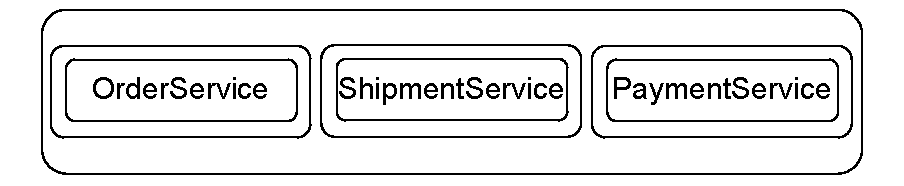
\includegraphics[scale=0.70]{imglib/mono/mono-example}
        \caption{E-Commerce-Beispiel mit Modular Monolithic Architecture}
        \label{fig:mono-modular}
    \end{figure}
\end{frame}

\begin{frame}{Modular Monolithic Architecture: Agilität}
    \begin{itemize}
        \item Im Vergleich zu Monolith: Verbesserungen bezüglich Entwicklung
        \begin{itemize}
            \item Reduzierte Komplexität $\Rightarrow$ bessere Wartbarkeit
            \item Modularisierung ermöglicht kleine semi-autonome Teams
        \end{itemize}
        \item Noch immer problematisch:
        \begin{itemize}
            \item Deployment im Ganzen
            \item Keine horizontale Skalierung
            \item Keine Wiederverwendbarkeit von Funktionalitäten
        \end{itemize}
    \end{itemize}
\end{frame}
